%%%%%%%%%%%%%%%%%%%%%%%%%%%%%%% SECCIÓN 4 - DOCKER BUILD-RUN-RM %%%%%%%%%%%%%%%%%%%%%%%%%%%%%%%
\subsection{Construcción, ejecución y eliminación de los tres contenedores.}

\subsubsection{Construcción de los tres contenedores}
\par Para construir los tres contenedores con tres imágenes diferentes en el mismo directorio con distintos \texttt{Dockerfile},
tengo que indicar un nombre de imagen diferente a cada una y otro a cada fichero \texttt{Dockerfile}.
Para ello utilizo el comando \texttt{docker build [-t|--tag] [nombre-imagen-resultante] [-f nombre-dockerfile] .} como se muestra en la Figura \ref{fig:docker-build}.
%%% IMAGEN DOCKER BUILD %%%
\begin{figure}[H]
    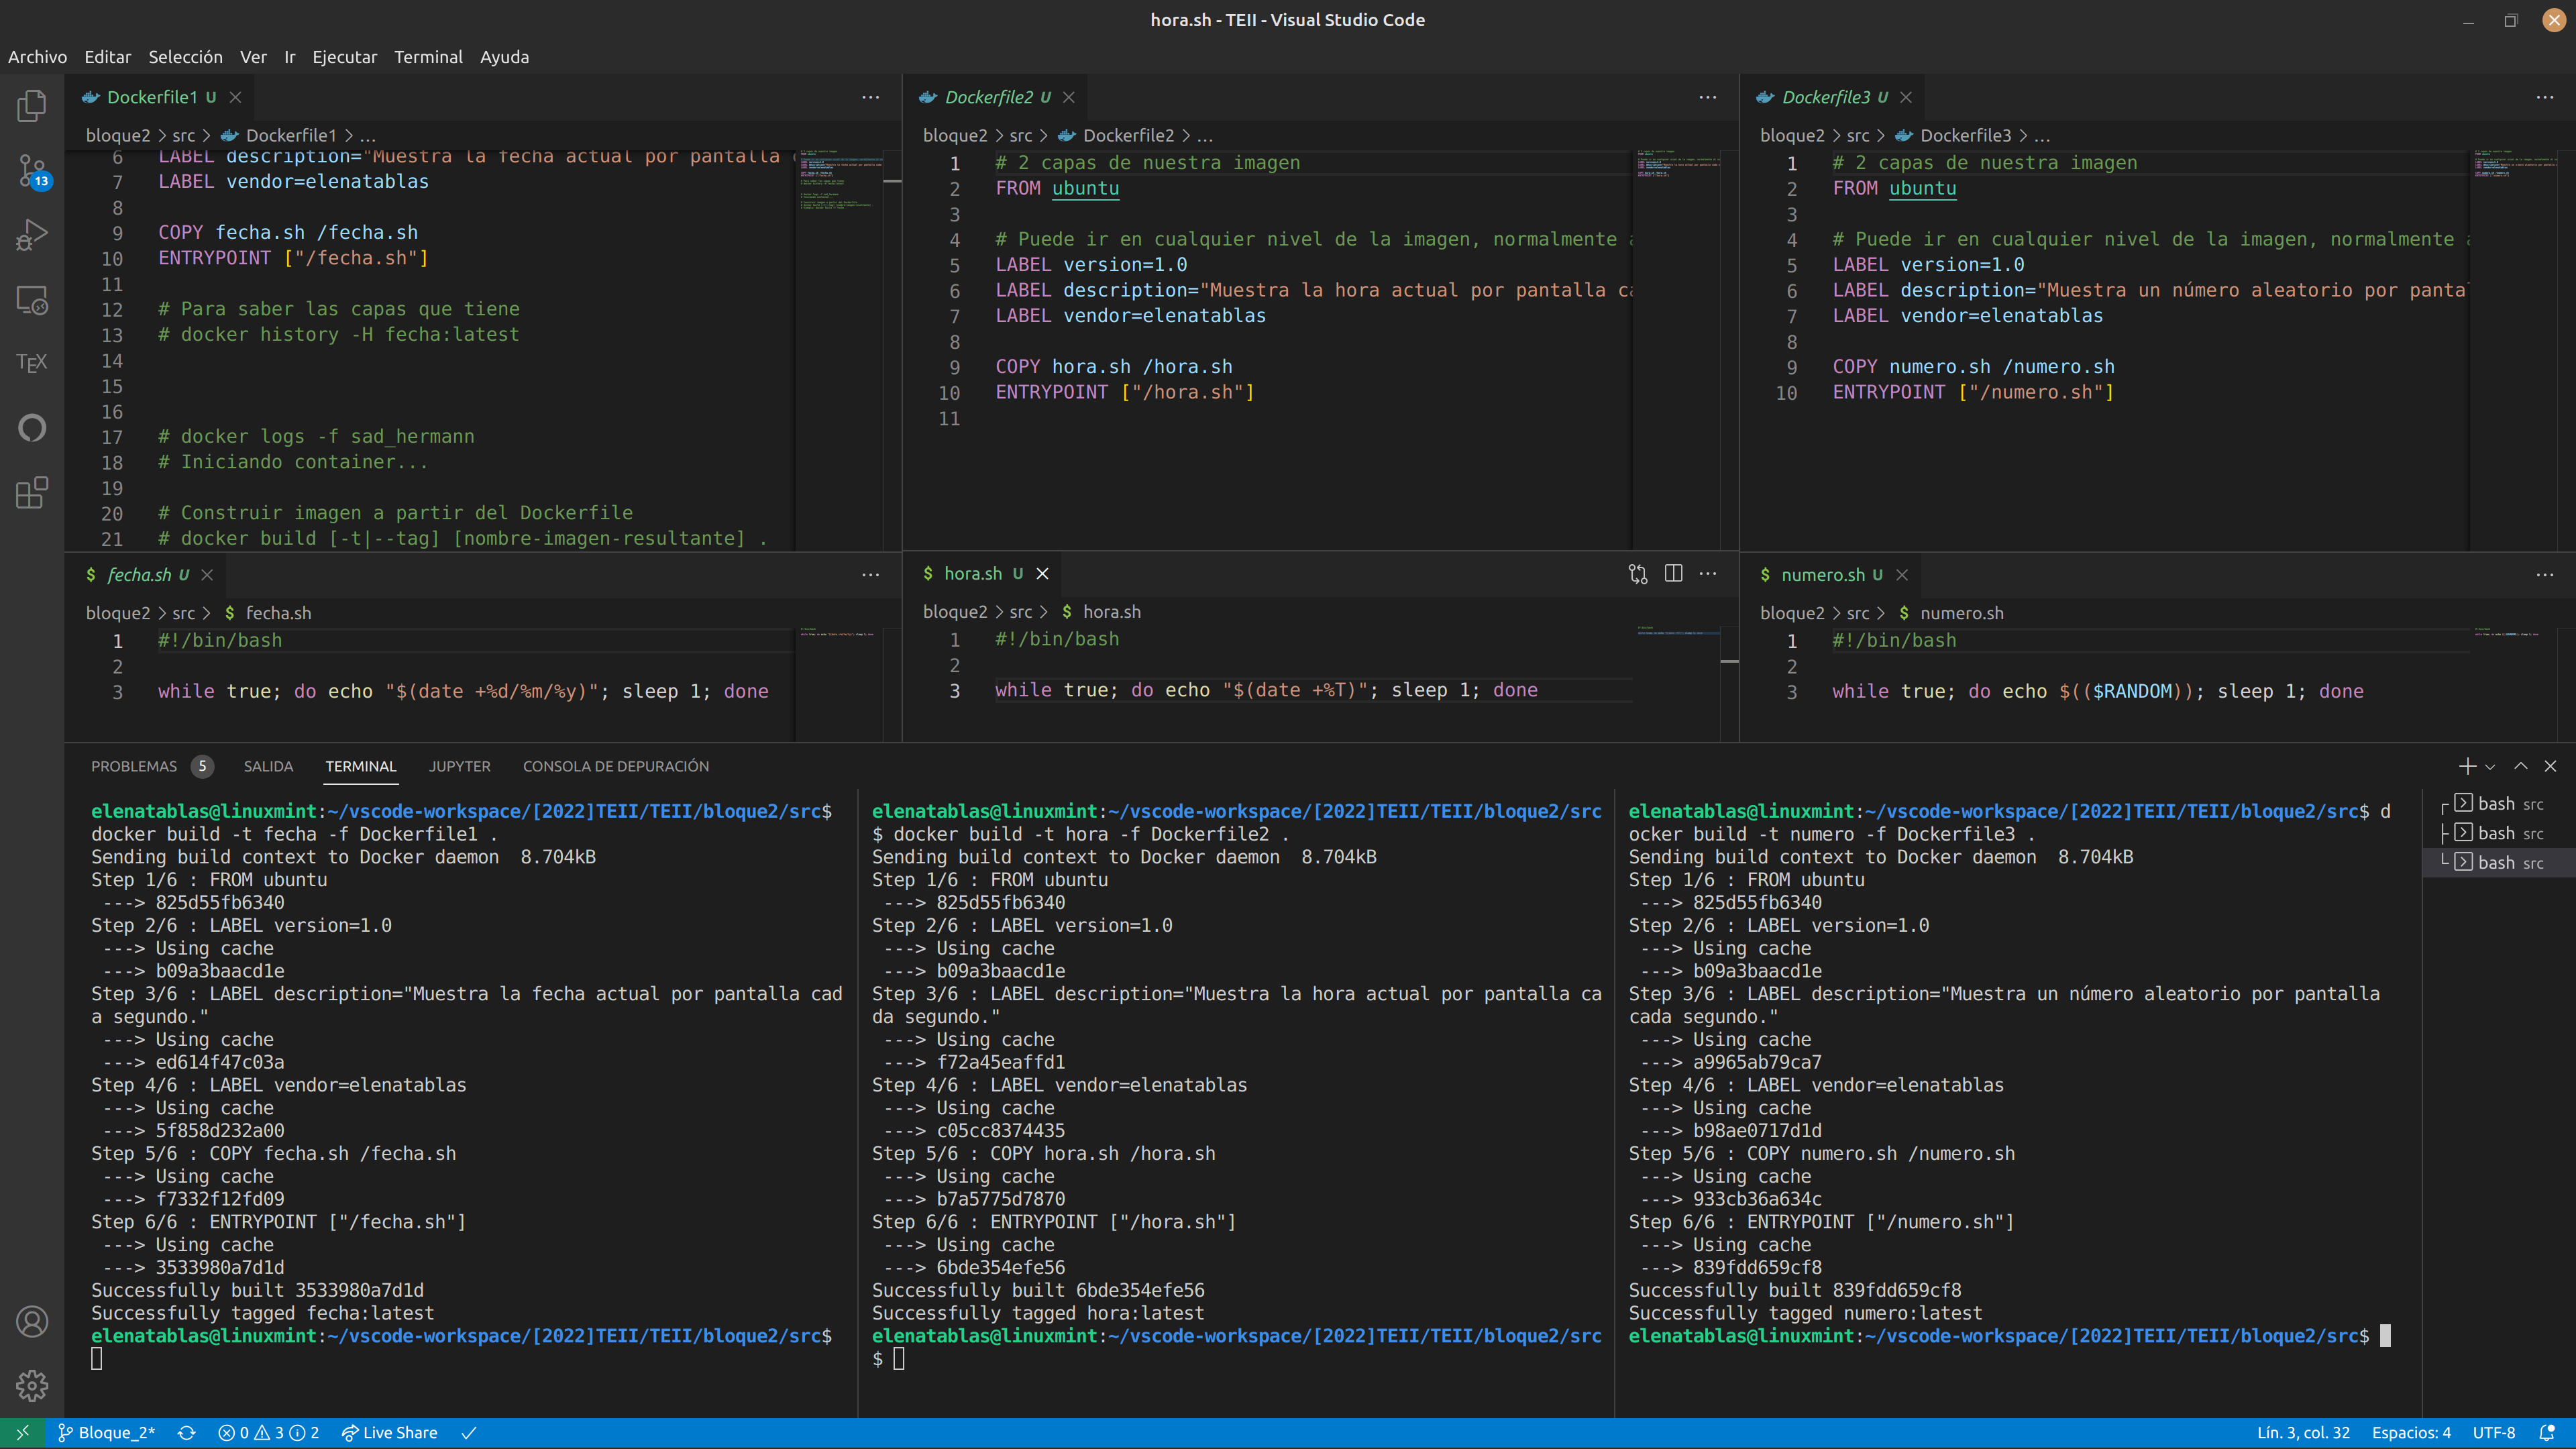
\includegraphics[width=\textwidth]{docker-build}
    \centering
    \caption{Construcción de los tres contenedores al mismo tiempo.}
    \label{fig:docker-build}
 \end{figure}

\newpage

\subsubsection{Ejecución de los tres contenedores}
\par Se puede observar como los tres contenedores se ejecutan 
a la vez cada segundo tal y como indica el segundo contenedor en la Figura \ref{fig:docker-run}
y los resultados son los esperados.

%%% IMAGEN DOCKER RUN %%%
\begin{figure}[H]
   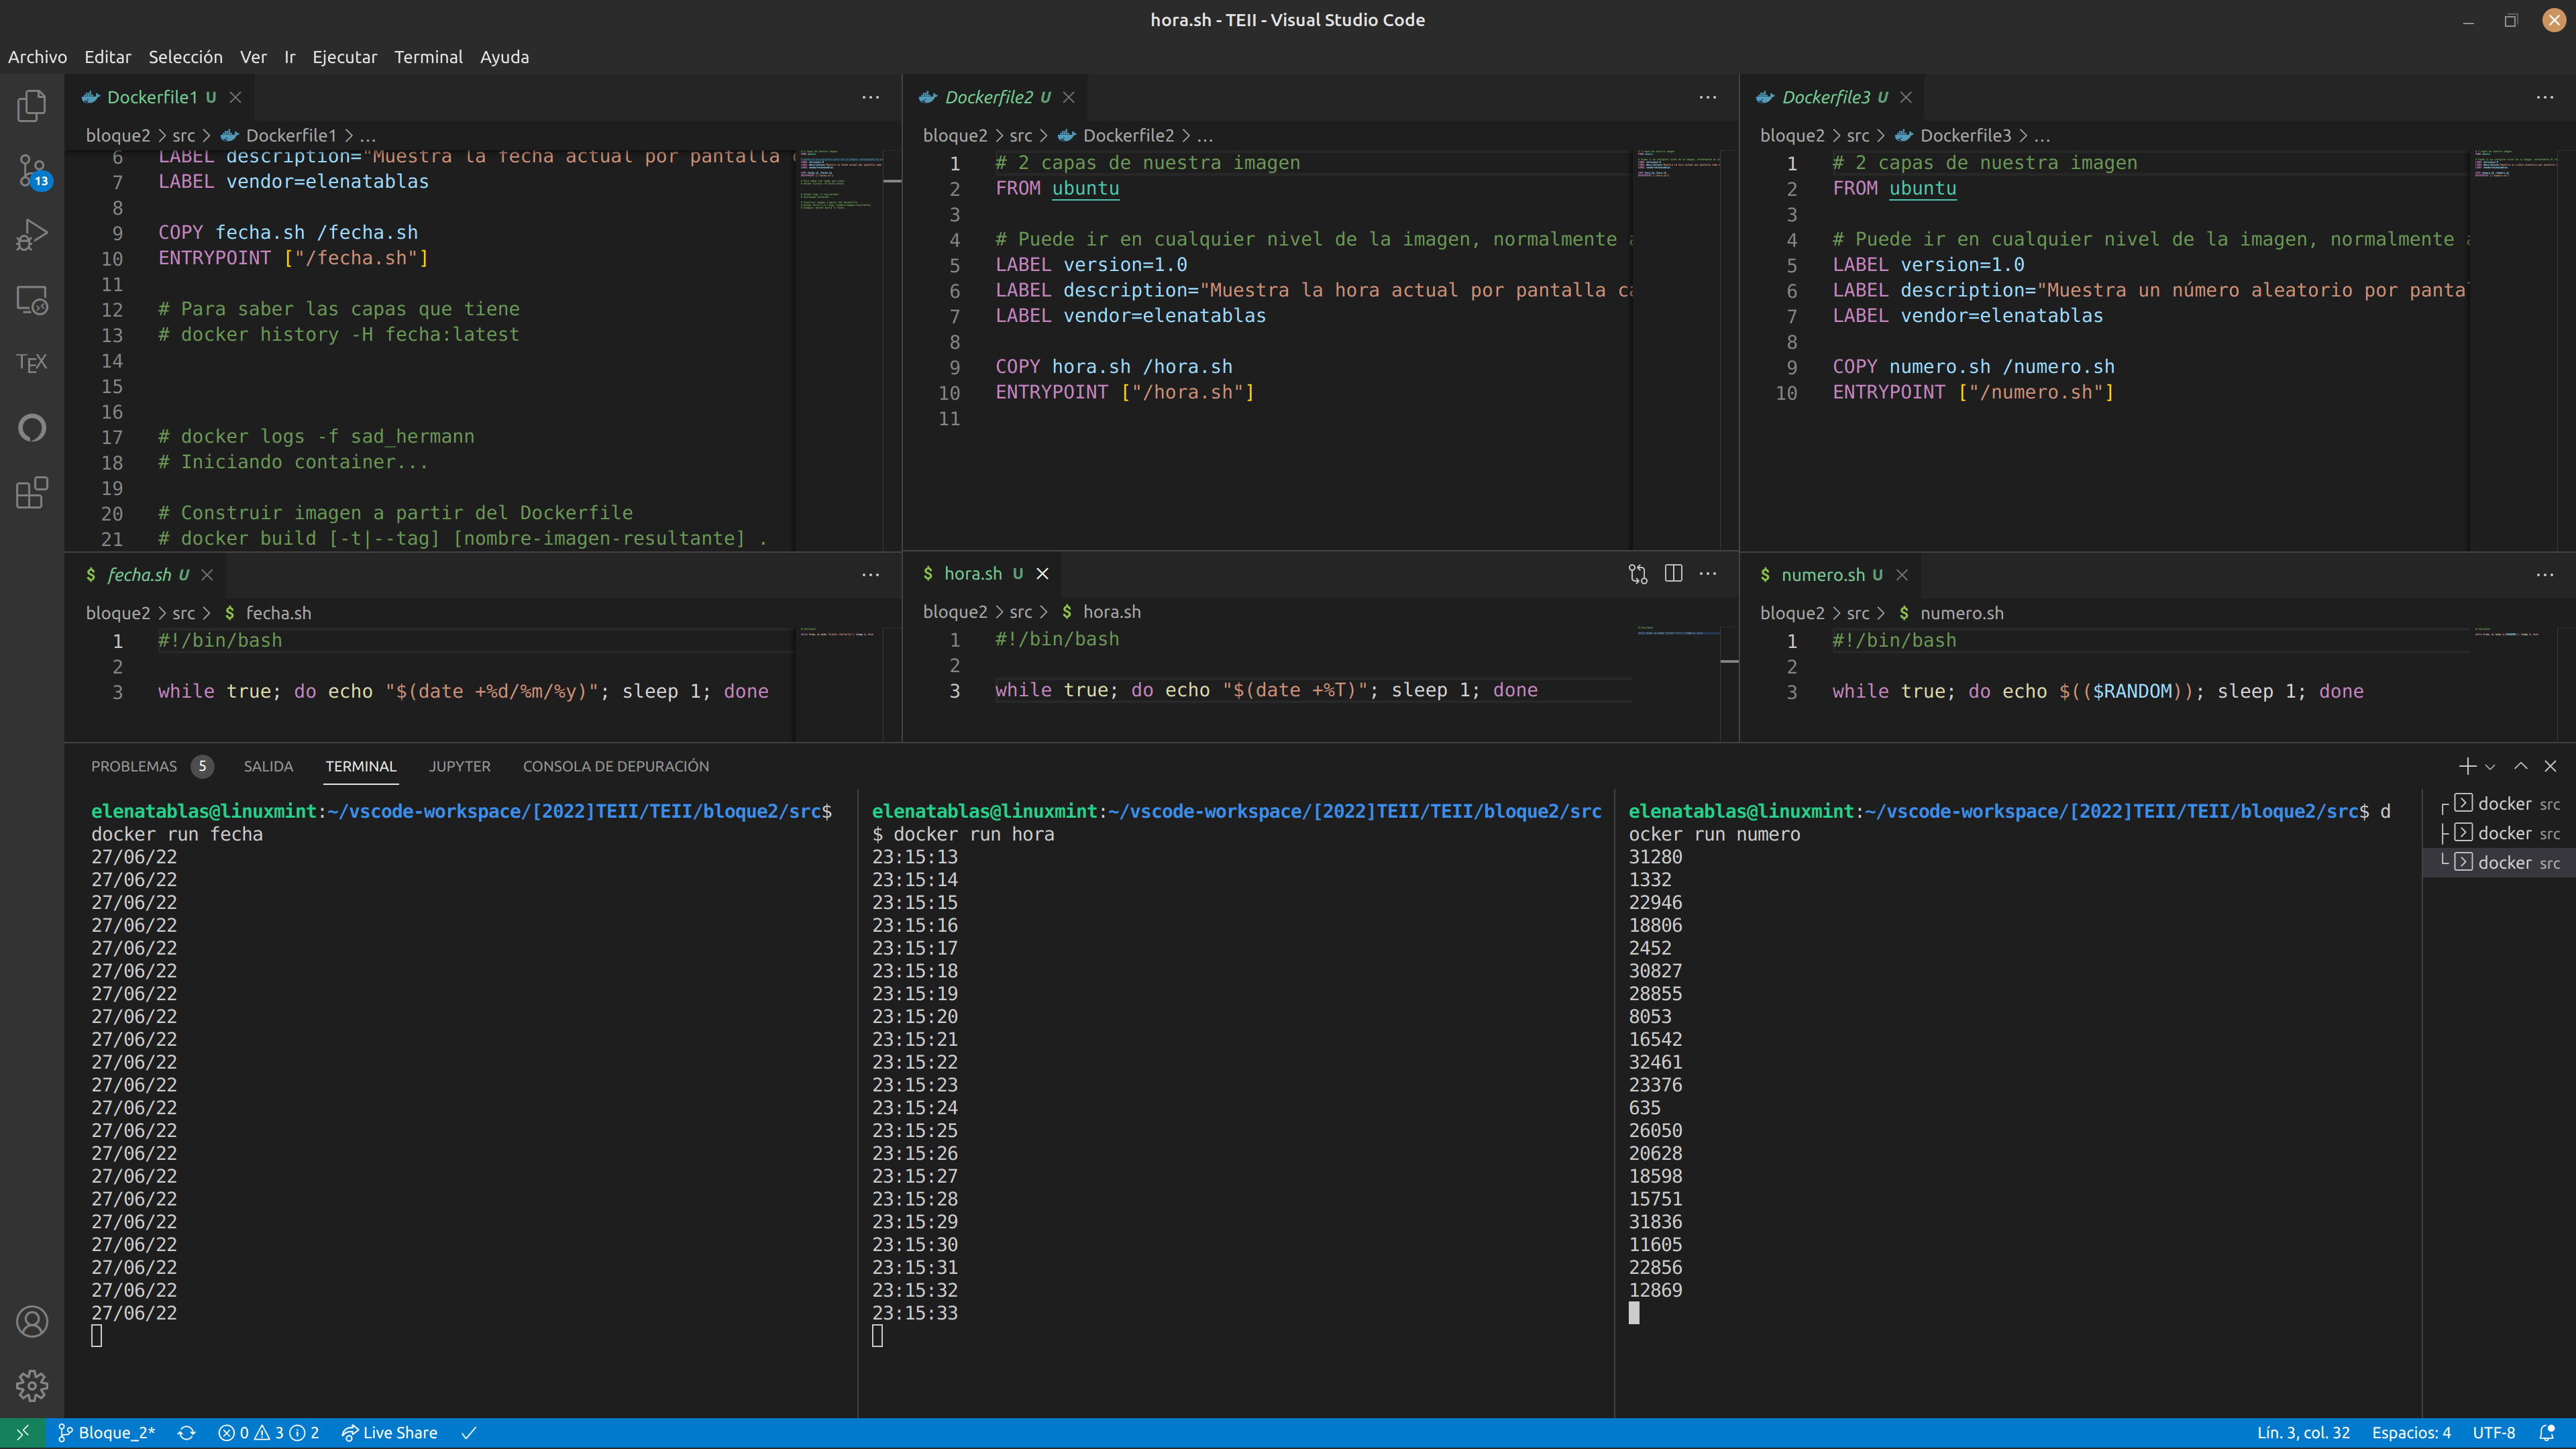
\includegraphics[width=\textwidth]{docker-run}
   \centering
   \caption{Ejecución de los tres contenedores al mismo tiempo.}
   \label{fig:docker-run}
\end{figure}


\subsubsection{Eliminación de los tres contenedores}
\par Primero, listo todos los contenedores que están en ejecución o detenidos. Segundo, 
identifico cuales son los que quiero eliminar, que como se puede observar en la Figura 
\ref{fig:docker-rm} son los únicos procesos que existen y los puedo borrar tanto por tu id
como por el nombre asignado por defecto. Los elimino sin contemplar su estado los tres a la vez.
 %%% IMAGEN DOCKER RM %%%
 \begin{figure}[H]
	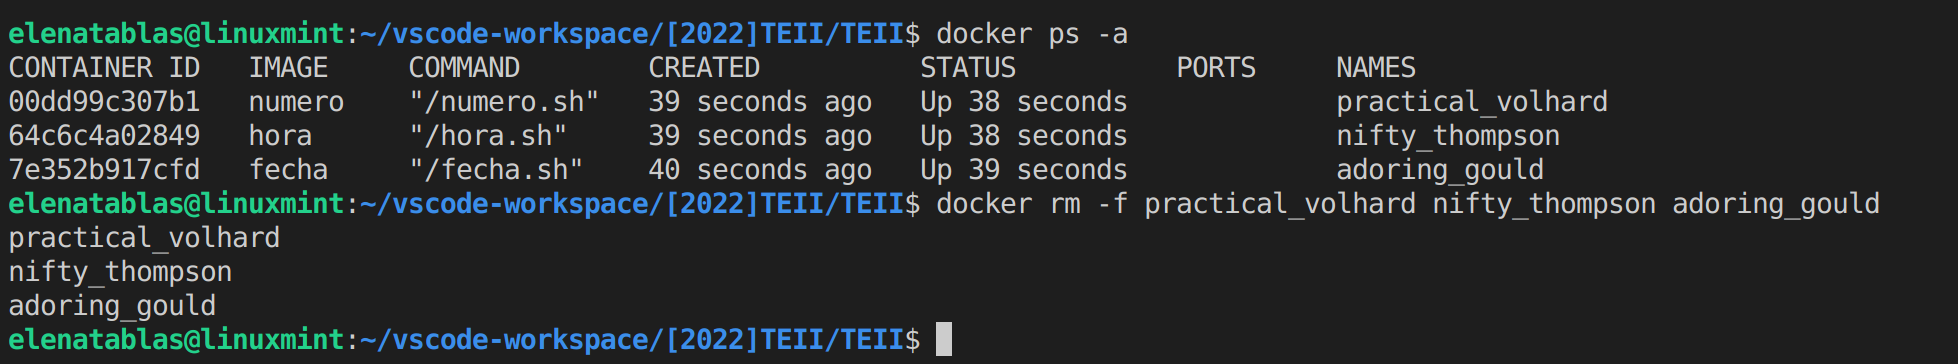
\includegraphics[width=\textwidth]{docker-rm}
	\centering
	\caption{Eliminación de los tres contenedores al mismo tiempo.}
    \label{fig:docker-rm}
\end{figure}